\documentclass[../../main.tex]{subfiles}
\begin{document}
\begin{oframed}
  \subfile{problem}
\end{oframed}

{\bf [解答]}

\paragraph{(1)}

与えられた関数
\begin{align}
  f(x) = \log (x+\sqrt{1+x^2})
\end{align}
の両辺$x$で微分して
\begin{align}
  f'(x)=\dfrac{1}{\sqrt{1+x^2}}
\end{align}
である．

\paragraph{(2)}

\begin{figure}[htb]
  \centering
  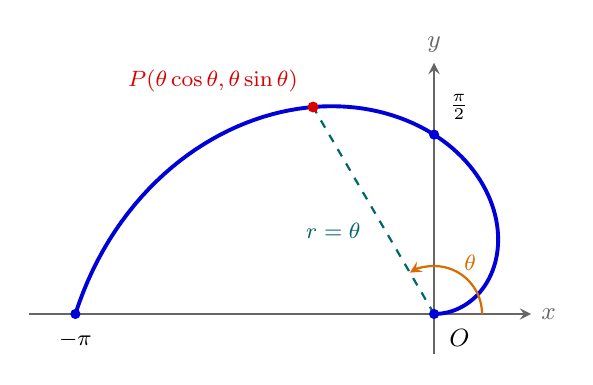
\begin{tikzpicture}[x=1.45cm, y=1.45cm, >=stealth, every node/.style={font=\small}]
    \coordinate (O) at (0,0);
    \draw[->, thick, gray!80!black] (-3.55,0) -- (0.85,0) node[right] {$x$};
    \draw[->, thick, gray!80!black] (0,-0.35) -- (0,2.2) node[above] {$y$};
    % アルキメデスの渦巻線 r = theta (0 <= theta <= pi)
    \draw[line width=1.4pt, blue!85!black, domain=0:3.14159, samples=100]
    plot ({\x*cos(\x r)}, {\x*sin(\x r)});
    % 代表点 P (theta = 2.1 rad 付近)
    \pgfmathsetmacro{\th}{2.1}
    \coordinate (P) at ({\th*cos(\th r)}, {\th*sin(\th r)});
    \draw[dashed, teal!80!black, thick] (O) -- (P)
    node[midway, below left=1pt, font=\footnotesize, teal!80!black] {$r=\theta$};
    \draw[orange!85!black, thick, ->] (0.42,0) arc[start angle=0, end angle={deg(\th)}, radius=0.42];
    \node[font=\footnotesize, orange!85!black] at (55:0.55) {$\theta$};
    % 特徴点 O(0,0), (0, pi/2), (-pi, 0), P
    \node[circle, fill=blue!85!black, inner sep=1.3pt] at (O) {};
    \node[circle, fill=blue!85!black, inner sep=1.3pt] at (0,1.5708) {};
    \node[circle, fill=blue!85!black, inner sep=1.3pt] at (-3.14159,0) {};
    \node[circle, fill=red!85!black, inner sep=1.4pt] at (P) {};
    \node[below right=2pt] at (O) {$O$};
    \node[above right=2pt, font=\footnotesize] at (0,1.5708) {$\frac{\pi}{2}$};
    \node[below=3pt, font=\footnotesize] at (-3.14159,0) {$-\pi$};
    \node[above left=2pt, red!85!black, font=\footnotesize] at (P) {$P(\theta\cos\theta,\theta\sin\theta)$};
  \end{tikzpicture}
  \caption{曲線$r=\theta$（$0\le\theta\le\pi$）の概形}
  \label{fig:spiral_curve}
\end{figure}

題意の曲線$C$上の点は$
\begin{pmatrix}x\\y
\end{pmatrix}=\theta
\begin{pmatrix}\cos\theta\\\sin\theta
\end{pmatrix}$と表せるから，もとめる長さ$L$として
\begin{align}
  L&=\int_0^\pi\sqrt{\left(\dfrac{dx}{d\theta}\right)^2+\left(\dfrac{dy}{d\theta}\right)^2}\,d\theta\\
  &=\int_0^\pi\sqrt{(\cos\theta-\theta\sin\theta)^2+(\sin\theta+\theta\cos\theta)^2}\,d\theta\\
  &=\int_0^\pi\sqrt{1+\theta^2}\,d\theta\\
  &=\dfrac{1}{2}\left[\theta\sqrt{1+\theta^2}+\log\left(\theta+\sqrt{1+\theta^2}\right)\right]_0^\pi\\
  &=\dfrac{1}{2}\left\{\pi\sqrt{1+\pi^2}+\log\left(\pi+\sqrt{1+\pi^2}\right)\right\}
\end{align}
である．

\newpage

\end{document}
